\documentclass{jbsc}

\begin{document}

\title{On Cluster Robust Models}
\author{José Bayoán Santiago Calderón\thanks{Santiago Calderón: Claremont Graduate University, \href{mailto:naoyabpr@gmail.com}{naoyabpr@gmail.com}.}}
\date{\today}

\maketitle

\begin{abstract}
Empirical work commonly deals with heterogeneous in treatment populations with potential clustered sampling design. Current approaches to overcome issues that arise in these cases include weighted least squares, fixed effects models, and cluster robust variance covariance estimators. However, the current solutions often offer sub-optimal performance or practitioners misuse them. This study examines possible disadvantages to using non-cluster robust models and alternative solutions. Some of the contributions include a framework to understand and develop cluster robust models with new advise for practitioners and practical considerations. (JEL C01)
\end{abstract}

Cluster robust models refer to statistical models that attempt inference about a heterogeneous in treatment population. A common target for estimation is the average treatment effect (ATE), which is defined as the average marginal effect of each observation in the population. Models with homogeneous in treatment populations have an universal marginal effect for all observations in the population leading to the marginal effect being identical to the ATE. However, when there are multiple marginal effects, these models have clusters, which are defined as a subgroup of observations with the same marginal effect. Obtaining a good estimate for the ATE requires: (1) a representative sample or additional cluster specific information, (2) an appropriate model / estimator for the model parameters, and (3) a correct estimator for the second moment.

Most of the studies about cluster robust models takes place in the context of longitudinal data. Estimators typically employed in panel data settings are pooled ordinary least squares, between, least squares dummy variables / within estimator (fixed effects model), and random effects. However, cluster robust models are prevalent in cross sectional studies, especially in experimental studies, but common in observational as well. One of the most frequent estimators, the fixed effects model, assumes the following data generation process
\begin{equation}
y = \alpha_{g} + X \beta + u
\end{equation}
where $y$ is the outcome variable, $\alpha_{g}$ the cluster specific intercept term, $X$ the linear predictor, $\beta$ the model parameters, and $u$ the idiosyncratic error term. However, this estimator is generally inconsistent or very biased for ATE in the case of heterogeneous in treatment effects populations as it assumes an incorrect data generation process \citep{Gibbons_SúarezSerrato_Urbancic_2018}. Cluster robust variance covariance estimators (CRVE) \citep{Liang_Zeger_1986, Arellano_1987, Rogers_1993, Cameron_Gelbach_Miller_2011}, typically used with the within estimator or random effects models,  assume heterogeneous in treatment effects which results in using a potential appropriate variance covariance estimator for an assumed inconsistent estimator of the model parameters \citep{Abadie_Athey_Imbens_Wooldridge_2017}. This is akin to using an heteroscedasticity consistent (HC) variance covariance estimator \citep{Eicker_1967, Huber_1967, White_1980, MacKinnon_White_1985} for logit or probit models which implies assuming an incorrect specification of the first moments \citep{Wooldridge_2010}. Nevertheless, CRVE are typically employed in fixed effects models since HC variance covariance estimators can be inconsistent for short panels under very reasonable assumptions \citep{Stock_Watson_2008}.

The data generation process for a bi-dimensional model with heterogeneity in treatment for a single dimension can be characterized by
\begin{equation}
y = \alpha + X_{1} \left(\beta_{1} + \gamma_{g}\right) + X_{2} \beta_{2} + u
\end{equation}
where $y$ is the outcome variable, $X_{1}$ is the heterogeneous in treatment dimension, $X_{2}$ a homogeneous in treatment dimension, $\alpha$ is the intercept coefficient, $\beta_{k}$  and $\gamma_{g}$ are the model parameters with $\gamma_{g}$ being the heterogeneity in treatment parameters, and $u$ an idiosyncratic error term. In order to properly estimate the ATE for $X_{1}$, there are a few prerequisites best understood in the general inference for statistical models framework.

Two major approaches for causal studies include observational and randomized experiments \citep{Athey_Imbens_2016}. Observational studies do not rely on exploiting variation of the treatment mechanism, but do rely on the stochastic nature of the responses. Given a population of interest, an observational statistical model has a data generation process model and a sampling design that describes how samples are constructed based on the population of interest.

Given a sampling design, an estimator can be employed to obtain the main parameters, usually partial correlations of each feature, to approximate the average marginal effect of explanatory variables. In order for an estimator to have desirable properties, such as consistency and be low bias, the sample should be representative of the underlying population. Sampling design requires two major components: (1) each share of heterogeneous in treatment groups is proportional to its share in the population and (2) the distribution of the explanatory variables for each subgroup is representative \citep{Solon_Haider_Wooldridge_2015}. Absent a representative sample, one may be able to generate a representative sample using weights. A possible alternative is to obtain estimates of the treatment effects and rely on an estimated composition for the population to infer the ATE.

Variability or uncertainty of parameter estimates (point estimates) arise from the sampling design. In order to capture the uncertainty in the estimates, variance covariance estimates yield complimentary information about the distribution of the parameter estimates. Confidence intervals follow from the variance covariance estimates and an approximate distribution. Moreover, these components can be used for Wald-test applications such as hypothesis testing.

Heterogeneous in treatment populations are commonplace in applied work. For example, rates of the return on education might vary significant across socioeconomic and demographic dimensions. A classic question in such studies is whether the subgroups can or should be ``pooled''. The answer will depend on what insight one aims to gain (what are the parameters of interest) and the bias-variance trade-off resulting from choosing one model over the other \citep{Baltagi_2013}. When using an unrestricted model, some subgroups will have different partial correlations in some dimensions that may affect the consistency, bias, rate of convergence, and variance of the estimator.

Assuming no clustered treatment assignment, cluster robust variance covariance estimators are correct when there is heterogeneity in treatment and clustered sampling \citep{Abadie_Athey_Imbens_Wooldridge_2017}. The usual cluster robust variance covariance estimator is a special case which provides approximate correct estimates under additional quite restrictive assumptions. This study uses advances in the literature of cluster robust models for first and second moments that yields new guidelines for practitioners.

\section{Proposed Estimator}

Consider the following data generation process
\begin{equation}
\label{model}
y = \beta_{0} + X_{1} \left(\beta_{1} + \gamma_{g}\right) + X_{2} \beta_{2} + u
\end{equation}
where $y$ is the outcome variables, $X_{1}$ and $X_{2}$ are explanatory variables, $\beta_{j}$ and $\gamma_{g}$ are the main parameters, and $u$ is the idiosyncratic error term. The data generation process indicates that the population of interest is heterogeneous in treatment, specifically in the $X_{1}$ dimension. Clusters $g \in G$ are determined by the relation between $X_{1}$ and $y$; meaning $\beta_{1} + \gamma_{g}$.

Modifying the regression model to estimate the heterogeneity parameters allows to learn both the parameter estimates and obtain correct estimates of the second moment for inference using only heteroscedasticity consistent variance covariance estimators. The ATE can be computed as a weighted linear combination of the estimates that properly accounts for the population composition.

\section{Methodology}

Consider model from equation \ref{model} and without loss of generality, let the explanatory variables as well as the error term be standard normal distributed $X_{1}, X_{2}, u \sim \mathcal{N}\left(0,1\right)$.\footnote{Some simulation studies adjust the variance of the explanatory variables by cluster as one potential way to incorporate heterogeneity in attributes. The simulations depend in heterogeneity of treatment effects for which, it considers an homogeneous in attributes population simplifying one of the requirements for obtaining representative samples.} As for the main parameters, $\left(\beta_{1}, \beta_{2}\right) = \left(1, 0.5\right)$ and
\begin{equation}
\gamma_{g} =
\begin{cases}
- 0.50 & \text{ if } g = 1\\
- 0.25 & \text{ if } g = 2\\
\ \ 0.00 & \text{ if } g = 3\\
\ \ 0.25 & \text{ if } g = 4\\
\ \ 0.50 & \text{ if } g = 5
\end{cases}
\end{equation}
which yields
\begin{equation*}
    \left(\beta_{1} + \gamma_{1}, \beta_{1} + \gamma_{2}, \beta_{1} + \gamma_{3}, \beta_{1} + \gamma_{4}, \beta_{1} + \gamma_{5}\right) = \left(0.50, 0.75, 1.00, 1.25, 1.50\right)
\end{equation*}.
The population is finite with 100,000 observations and each observation is assigned a subgroup $g \in \left\{\mathbb{Z}\,|\,g \in [1, 5]\right\}$ with equal probability. The least squares solution to the following model
\begin{equation}
\label{naiveformula}
y \sim X_{1} + X_{2}
\end{equation}
using the entire population leads to $\hat{\beta} \approx \left(0.0059, 0.9996, 0.5037\right)$ which is not surprising given the heterogeneity in treatment effect distribution and the uniform probability distributed shares of each group in the population.

The first sampling design is random sampling which assigns each observation in the population a 10\% probability of being observed in each sample draw. The alternative sampling design is clustered sampling which assigns a cluster dependent probability of any observation being observed in a sample draw. Each trial will randomly assign one the following elements to each subgroup without replacement $\left\{0.10, 0.15, 0.20, 0.25, 0.30\right\}$ as the subgroup dependent probability of being observed for each member observation. The clustered sampling may be implied by stratified sampling as assigning different subgroup probabilities to various subgroups eventually define the probability of being sampled by each cluster.

During each trial, a sampling process determines which observations are observed. In the first stage, the formula used to fit the regression model is equation \ref{naiveformula}. In addition to estimating the main parameters, the HC1 and CRVE are computed using a perfect information setting (i.e., it uses the cluster membership dimension for the clustering). For each condition, 1,000 trials are performed and used to compute the coverage rate / empirical rejection rates for each non-intercept parameter. Given the sampling designs need not guarantee that the samples are representative, coverage rates are computed using the values in the data generation process as well as the empirical probability limit from 10,000 trials. Since the coverage rates do not change the overall results of the experiment the results reported are those using the data generation values and the results using the empirical probability limits are reported in the appendix.

\begin{table}[hbpt]
	\centering
    \caption{Results for Conventional Approach}
	\label{Conventional}
	\begin{threeparttable}
	\begin{tabularx}{\textwidth}{Y Y Y}
		\toprule
		& \textbf{Random}       & \textbf{Clustered} \\
		\midrule
		\textbf{HC1}  & 0.966, 0.946 & 0.175, 0.947 \\
		\textbf{CRVE} & 0.999, 0.944 & 0.300, 0.951\\
		\bottomrule
	\end{tabularx}
	\begin{tablenotes}
		\small
		\item The values reported are the coverage rates at the 0.95 confidence for $\hat{\beta}_{1}, \hat{\beta}_{2}$.
		\item The various conditions vary in sampling design and variance covariance estimators.
		\item The coverage rates are obtained from 1,000 trials.
	\end{tablenotes}
\end{threeparttable}
\end{table}

Under random sampling the probability limits match the weighted average treatment effects and the heteroscedasticity consistent estimator is appropriate. Meanwhile, using the cluster robust variance covariance estimator leads to overly conservative estimates for the confidence intervals of heterogeneous in treatment parameters and accurate for the remaining parameter estimates. Given a clustered sampling design, both variance covariance estimators provide close to nominal coverage rates for non-heterogeneous parameter estimates, but wrong estimates for the parameters that are heterogeneous in treatment.

\begin{figure}[hbpt]
	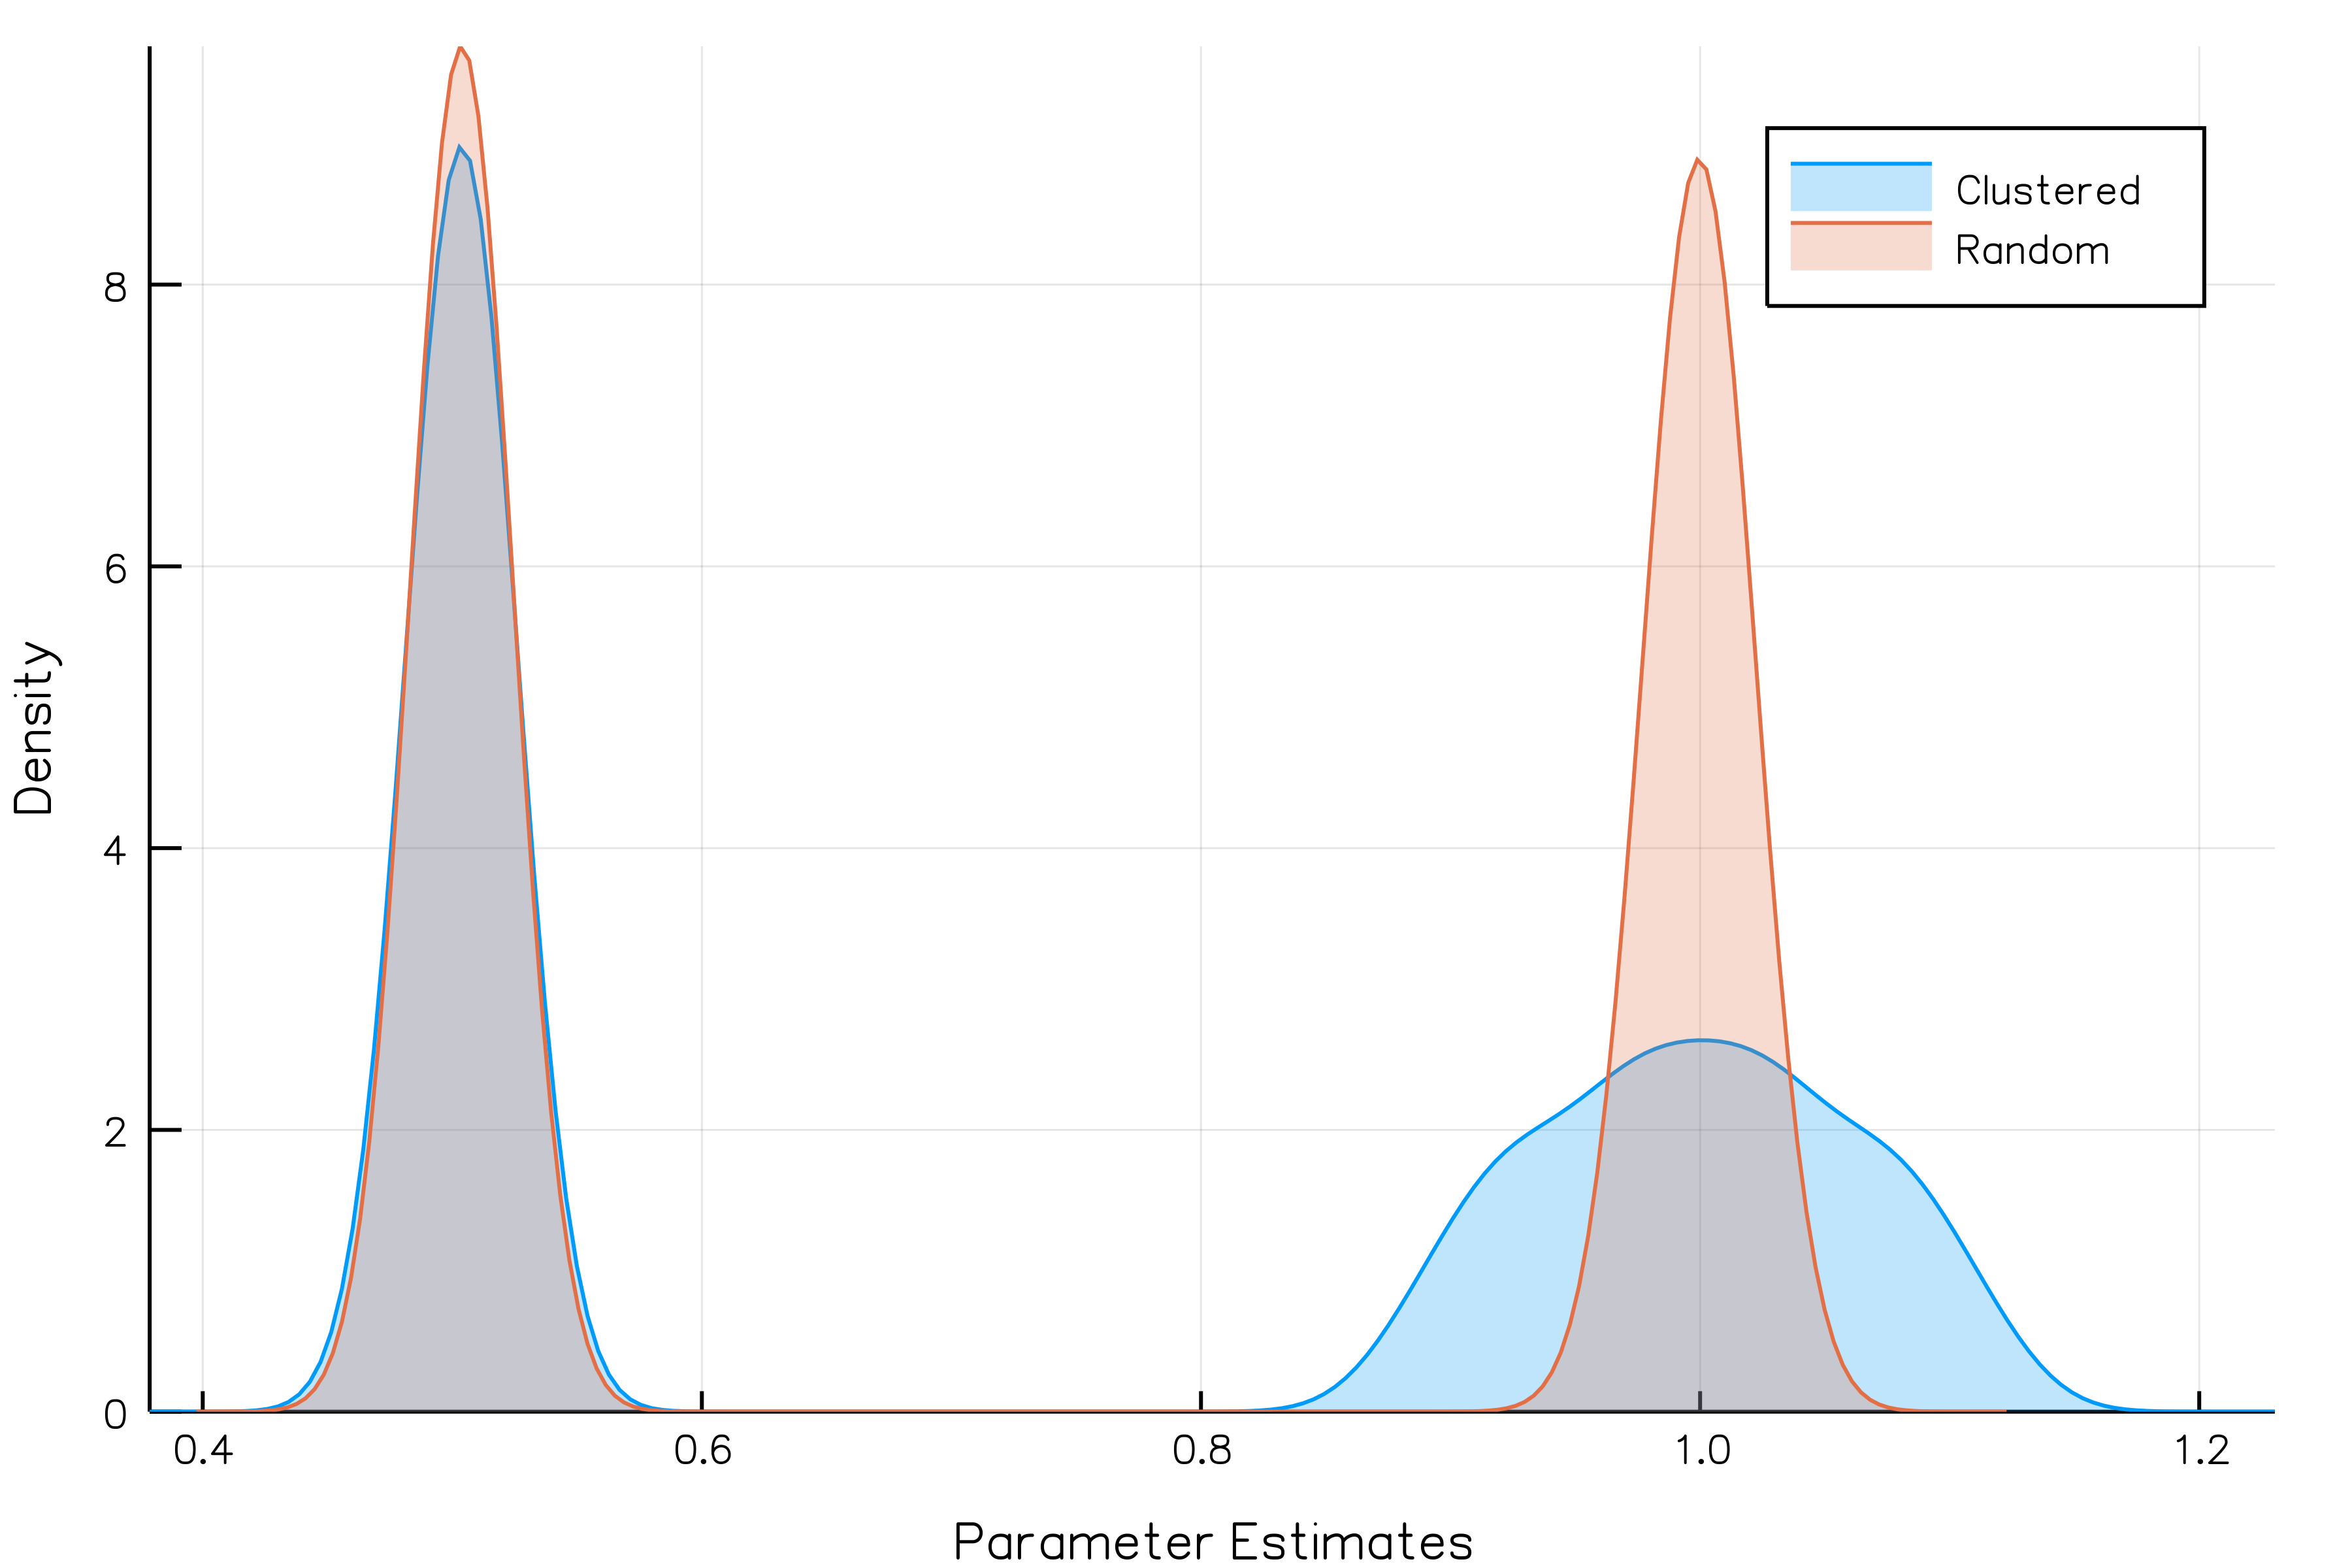
\includegraphics[width = \textwidth]{EPL.png}
	\caption{Distribution of Parameter Estimates (10,000 replications)}
	\label{EPL}
\end{figure}

Examining the distribution of parameter estimates shows that for the heterogeneous in treatment parameter the distribution between sampling designs is dramatically different (see Figure \ref{EPL}). Since the various cluster specific sampling probabilities are not fixed and vary for each trial, the probability limit is the same as random sampling, but the convergence rates are very different.

Following the failure of current variance covariance estimators to provide a valid tool answer to these kind of problems, what alternatives are there available? One possible venue could be to use weights in order to obtain a representative sample post-sampled (i.e., inverse probability weights). However, the proposed solution does not require estimating weights to obtain a representative sample. One may adjust the formula for the regression model in a way that takes into account the assumed heterogeneity in treatment.
\begin{equation}
y \sim X_{1} + X_{1}\,\&\,G + X_{2}
\end{equation}
where $a\,\&\,b$ is short-hand for the interaction effects and $G$ is a categorical variable indicating the cluster membership. Notice that the proposed model is different from a fixed effects model in that the fixed effects assumes uncorrelated cluster specific errors while the proposed model assumes heterogeneity in treatment in the $X_{1}$ dimension.

\begin{table}[hbpt]
	\centering
	\caption{Results for Proposed Estimator}
	\label{ProposedEstimator}
	\begin{threeparttable}
	\begin{tabularx}{\textwidth}{Y Y Y}
		\toprule
		& \textbf{Random} & \textbf{Clustered}     \\
		\midrule
		\textbf{HC1}  & 0.966, 0.946 & 0.175, 0.947 \\
		\textbf{CRVE} & 0.999, 0.944 & 0.300, 0.951 \\
		\bottomrule
	\end{tabularx}
	\begin{tablenotes}
		\small
		\item The values reported are the coverage rates at the 0.95 confidence for $\hat{\beta}_{1}, \hat{\beta}_{2}$.
		\item The various conditions vary in sampling design and variance covariance estimators.
		\item The coverage rates are obtained from 1,000 trials.
	\end{tablenotes}
\end{threeparttable}
\end{table}

Table \ref{ProposedEstimator} shows that using the proposed estimator yields superior results in terms of the parameter estimates and has the added benefit of \textit{un-clustering} the correlation structure for obtaining good components for Wald-test applications.

\section{Nuance on the Method}

A few advantages of the method includes disentangling the heterogeneous effects for the various subgroups which is in many applications a useful insight. However, for computing the weighted average marginal effect in the population one has to obtain a sense of the share of each subgroups in the population. For example, consider a model for estimating the weighted average marginal effect of some emergency contraception pill. Several factors will influence the marginal effect such as the time in menstrual cycle. Nevertheless, assume that the heterogeneity in treatment is determined by how prompt the pill is taken after the incidence (e.g., within 24 hours, 48 hours, 72 hours, or later). The weighted average marginal effect can then be computed using the proposed approach and estimating the share of subgroups in the population. The same additional assumption of representative distribution of explanatory variables by subgroups is needed regardless of which approach one selects (e.g., if the subgroup that takes the emergency contraception pill most promptly is also the subgroup with the most fertile time in their menstrual cycle); the sampling design should capture the phenomenon of the probability limit of the estimator converging to the weighted average marginal effect in the population. One last set of assumptions needed for correctly employing the estimator is identifying the heterogeneous in treatment dimensions and having a good proxy for identifying the clusters.

Concerning the cluster robust variance covariance estimator for the proposed model, there would no longer be heterogeneity in treatment meaning that either cluster robust or heteroscedasticity consistent estimators will differ very little if any. One can still perform Walt-tests for the marginal effects by groups or unrestricted forms through Wald-tests on the linear combinations. Alternatively, one could estimate the base parameter and include the interactions with all but one subgroups as a way to test the trade-off between an unrestricted and cluster robust combination and the proposed approach. The approach still is limited by the same common assumptions needed for inference under other estimators / models such as obtaining a good estimate of the population composition, but relaxes certain assumptions and provides robust estimates under others.

Lastly, we build a case for the salience of this study. Differences in the average treatment effects computed from incorrect models do not provide correct estimates and in many cases these differ substantially from cluster robust models \citep{Gibbons_SúarezSerrato_Urbancic_2018}. Moreover, the importance of heterogeneous effects is often ignored with grave consequences. For example, \citet{Stapleton_Oseni_Bababekov_Hung_Chang_2018} found that the recommended initiating breast cancer screening age matches that of white women, but results in under-screening for non-white women for almost two decades. In this case, extrapolating from one subgroup to the population of interest was a mistake and disentangling heterogeneity between groups can lead to an improvement through group specific models.

\section{Relaxing the Perfect Information Assumption}

Cluster robust models typically assume perfect information where each observation in the sample is properly identified as a member of its cluster on every relevant dimension. However, in applied work it is rarely if ever the case and one must use a good approximation based both in theory and educated guesses. For example, a survey design might collect information about individuals by households. In this case, for certain dimensions it is sensible to assume that members of the same household might share the same marginal treatment effect for some dimensions and that information could lead to a suitable proxy.

Cluster proxies have certain properties that characterize their quality: (1) purity, (2) level, and (3) dimension. Consider a study on self-image and one of the explanatory variables being exposure and use of social media (e.g., instrumented by hours spent on social media per day). The population of interest is heterogeneous in treatment in the exposure and use of social media by age groups: (1) 18 - 25, (2) 26 - 45, and (3) 46+. The researcher does not know the true data generation process and has access to their ages; thus models it by specifying the following clusters: (1) 18 - 25, (2) 26 - 35, (3) 36 - 45, (4) 46 - 60, (5) 61+. The purity of a cluster measures the degree to which observations in a cluster are part of the same group and no foreign observations are included. Using the 5-groups proxy, the researcher is able to achieve perfect purity as every cluster would only contain members of the same cluster. In terms of the level, the proxy has an incorrect level since clusters have been desegregated (i.e., groups 2 and 3 should be together as well as groups 4 and 5). Lastly, the model should specify the clusters as proper of the social media exposure and use variable and  should not be employed with other dimensions.

The study presents a simulation survey of first and second moments results using cluster robust models and non-cluster robust models. Each model is compared under three sets of conditions: (1) varying the purity level, (2) different precision levels, (3) correct dimension specification.

\FloatBarrier
\section{Simulation Design}

All simulations use the following design with a data generation process as follows
\begin{equation}
\label{model2}
y = \beta_{0} + X_{1} \left(\beta_{1} + \gamma_{g}\right) + X_{2} \beta_{2} + u
\end{equation}
where $y$ is the outcome variables, $X_{1}$ and $X_{2}$ are explanatory variables, $\beta_{j}$ and $\gamma_{g}$ are the main parameters, and $u$ is the idiosyncratic error term. The data generation process indicates that the population of interest is heterogeneous in treatment, specifically in the $X_{1}$ dimension. Clusters $g \in G$ are determined by the relation between $X_{1}$ and $y$; meaning $\beta_{1} + \gamma_{g}$. The explanatory variables as well as the error term are standard normal distributed $X_{1}, X_{2}, u \sim \mathcal{N}\left(0,1\right)$.\footnote{Some simulation studies adjust the variance of the explanatory variables by cluster as one potential way to incorporate heterogeneity in attributes. The simulations depend in heterogeneity of treatment effects for which, it considers an homogeneous in attributes population simplifying one of the requirements for obtaining representative samples.} The main parameters, $\left(\beta_{1}, \beta_{2}\right) = \left(1, 0.5\right)$ and
\begin{equation}
\gamma_{g} =
\begin{cases}
- 0.50 & \text{ if } g = 1\\
- 0.25 & \text{ if } g = 2\\
\ \ 0.00 & \text{ if } g = 3\\
\ \ 0.25 & \text{ if } g = 4\\
\ \ 0.50 & \text{ if } g = 5
\end{cases}
\end{equation}
which yields
\begin{equation*}
    \left(\beta_{1} + \gamma_{1}, \beta_{1} + \gamma_{2}, \beta_{1} + \gamma_{3}, \beta_{1} + \gamma_{4}, \beta_{1} + \gamma_{5}\right) = \left(0.50, 0.75, 1.00, 1.25, 1.50\right)
\end{equation*}.
The population is finite with 100,000 observations and each observation is assigned a subgroup $g \in \left\{\mathbb{Z}\,|\,g \in [1, 5]\right\}$ with equal probability. The sampling design is clustered with each cluster-specific probability randomly chosen without replacement from 0.10,	0.15, 0.20, 0.25, and 0.30.

Each simulation performs an experiment based on repeating trial where a sample is drawn and the model is specified as
\begin{equation}
y = X_{1}\ \&\ G + X_{2}
\end{equation}
where $G$ is a categorical variable and \& represents the interaction operator. The model is fitted and the parameter estimates are recorded as well as the empirical rejection rates using the \textit{HC1} \citep{Eicker_1967, Huber_1967, White_1980, MacKinnon_White_1985} variance covariance estimator at the 95\% confidence level.

During each section a different procedure is used to construct $G$ which allows to examine the consequences varying conditions and emerging trade-offs for estimating and using a cluster structure. In order to test how purity affects the model, the varying purity condition perturbs $G$ using the following rule: with probability $1 - p$, where $p$ is the purity level, the cluster identifier is selected from a different cluster ID with probability proportional to the difference in treatment effect. In other words, an observation belonging to the cluster with treatment effect 1.25 ($g = 4$) has probability $\left(1,2,3,4,5\right) = \left(\frac{2(1 - p)}{34}, \frac{3(1 - p)}{68}, \frac{3(1 - p)}{34}, p, \frac{3(1 - p)}{34}\right)$ where $p$ is the purity level.\footnote{The values rise from making the relative probabilities proportional to the absolute distance between marginal effects.} This has the property of being a valid probability distribution (non-negative mutually exclusive probabilities that add up to one) and makes it more likely for a cluster to be mislabeled with a similar cluster than with a more different one (e.g., an observation belonging to age group 25-30 might be mislabeled more likely with the 31-35 than the 56-60 years old cluster). In the analysis of precision level conditions, $G$ is obtained by allowing each observation to be a member of two clusters restricted such all subgroups have perfect purity with equal probability.

\FloatBarrier
\section{Analysis for Purity Conditions}

Proxies for establishing cluster structures are not necessarily the true cluster structure in the data generation process. In most empirical work, one can use educated guesses that might have a sensible accuracy, but it is important to understand how the results vary based on the quality of the proxy. This simulation studied the distribution of parameter estimates for a cluster robust model. Figure \ref{PurityLevels} shows the distribution of parameters estimates for a homogeneous in treatment parameter in the top-left subplot and the distribution of the five clusters of a heterogeneous in treatment dimension in the remaining subplots.


\begin{figure}[hbpt]
	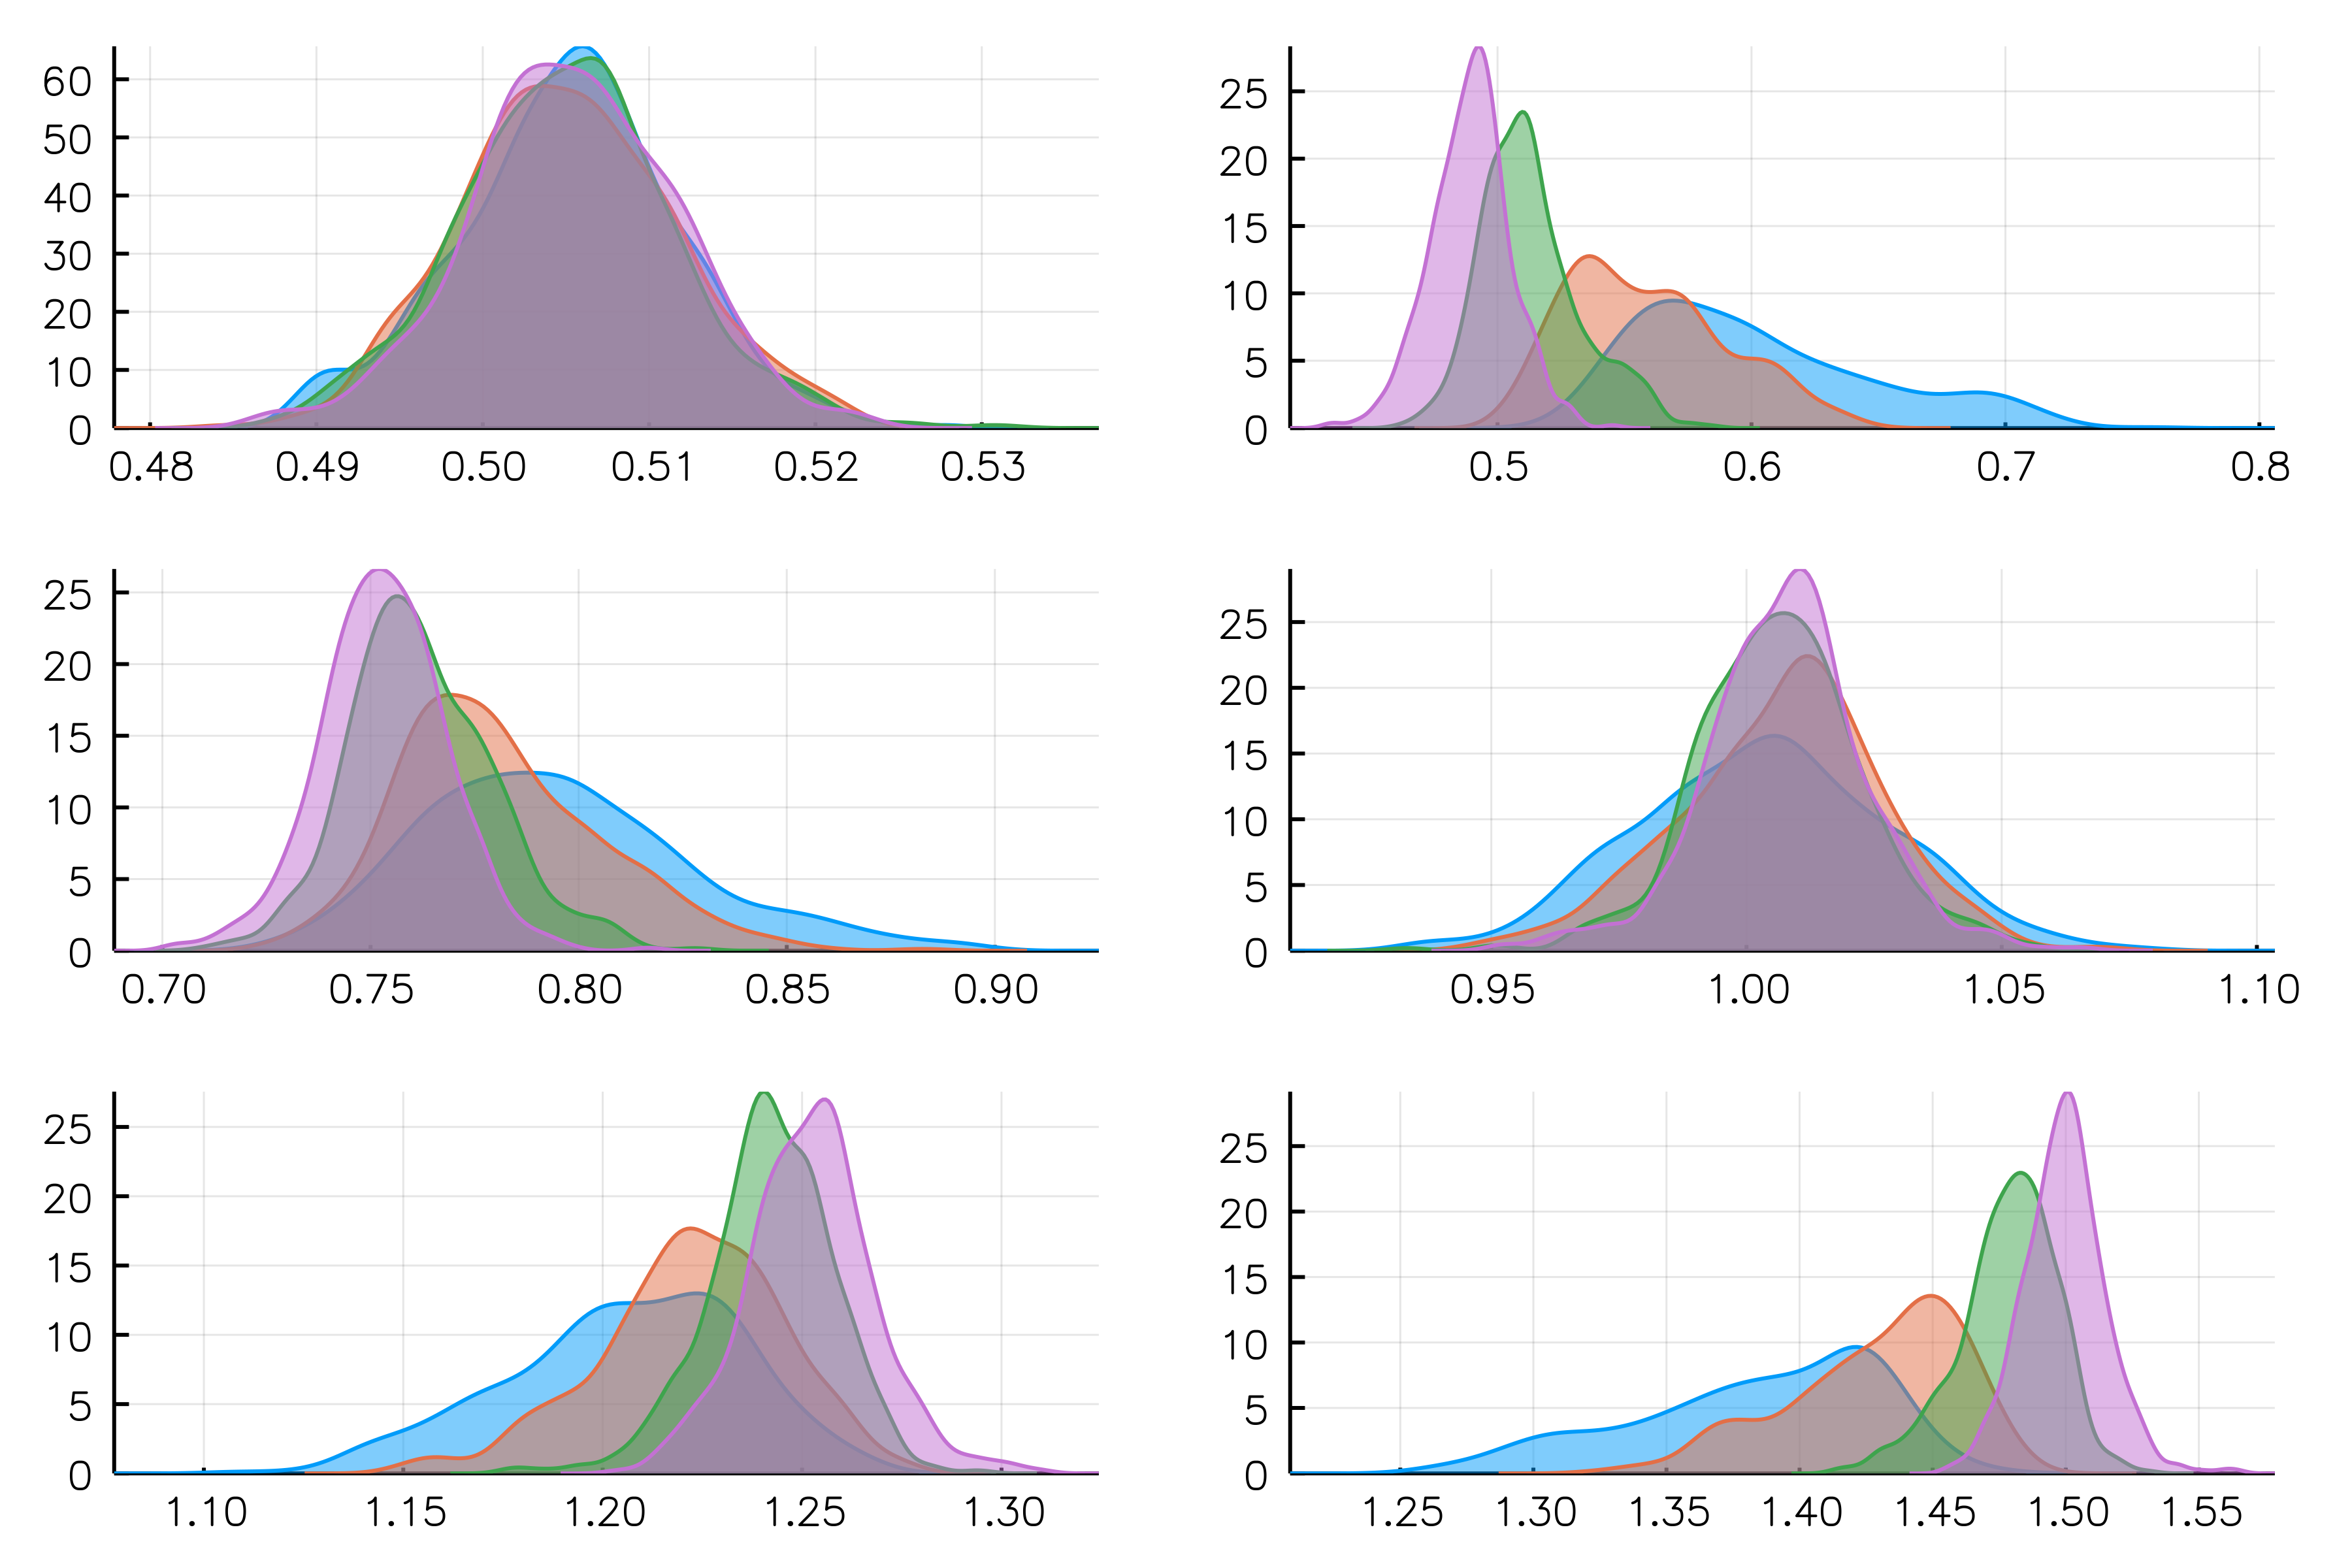
\includegraphics[width = 0.85\textwidth]{PurityPlots}
	\caption{Distribution of Parameter Estimates (500 replications)}
	\label{PurityLevels}
	{\footnotesize Note: The various purity levels shown are: 75\%, 85\%, 95\%, and 100\%.}
\end{figure}

The homogeneous in treatment parameter has a very similar distribution regardless of the level of purity. The level of purity in the heterogeneous in treatment set of parameters is very influential to the distribution of estimates. One can see that an incorrect cluster structure yields a distribution with skewness and and lower kurtosis than the normal distribution obtained from the correct specification. As a consequence, the variance covariance estimates obtained from cluster robust models are affected as well. Table \ref{EmpiricalRejectionRates} shows the progression of empirical rejection rates at the 95\% confidence level for selected expected purity levels: 75\%, 85\%, 95\%, and perfect information.

\begin{table}[hbpt]
	\centering
	\caption{Empirical Rejection Rates}
	\begin{threeparttable}
	\begin{tabularx}{\textwidth}{Y Y}
		\toprule
		\textbf{Parameter} & \textbf{Coverage Rate}\\
		\midrule
		$X_{1}$ \& G: 1 & 0.979 \\
		$X_{1}$ \& G: 2 & 0.961 \\
		$X_{1}$ \& G: 3 & 0.965 \\
	    $X_{1}$ \& G: 4 & 0.964 \\
	    $X_{1}$ \& G: 5 & 0.975 \\
	    $X_{2}$         & 0.978	\\
		\bottomrule
	\end{tabularx}
	\begin{tablenotes}
		\small
		\item Coverage rates for the 0.95 confidence level computed from 1e4 trials.
		\item The variance covariance estimator used was HC1, but using HC2 or HC3 may yield superior results and are consistent as the clustered nature has been dealt with within the primary estimator.
	\end{tablenotes}
\end{threeparttable}
	\label{EmpiricalRejectionRates}
\end{table}

\FloatBarrier
\section{Analysis for Precision Level Conditions}

Cluster robust models can be specified at a level that increases the probability of the proxy to being one of high purity. However, it may be the case that it leads to a large number of parameter estimates and difficult to obtain estimates of the population composition at that level of precision. An alternative is to estimate the model and use the results to develop a more parsimonious yet robust model based on the information gained.

Figure \ref{LowLevel} shows that a cluster robust model with pure proxies, but at the wrong level still provide consistent estimates. Moreover, the model results could be used to construct a refined proxy which uses the estimates of heterogeneous in treatment parameters for constructing a proxy at the correct level.

\begin{figure}[hbpt]
	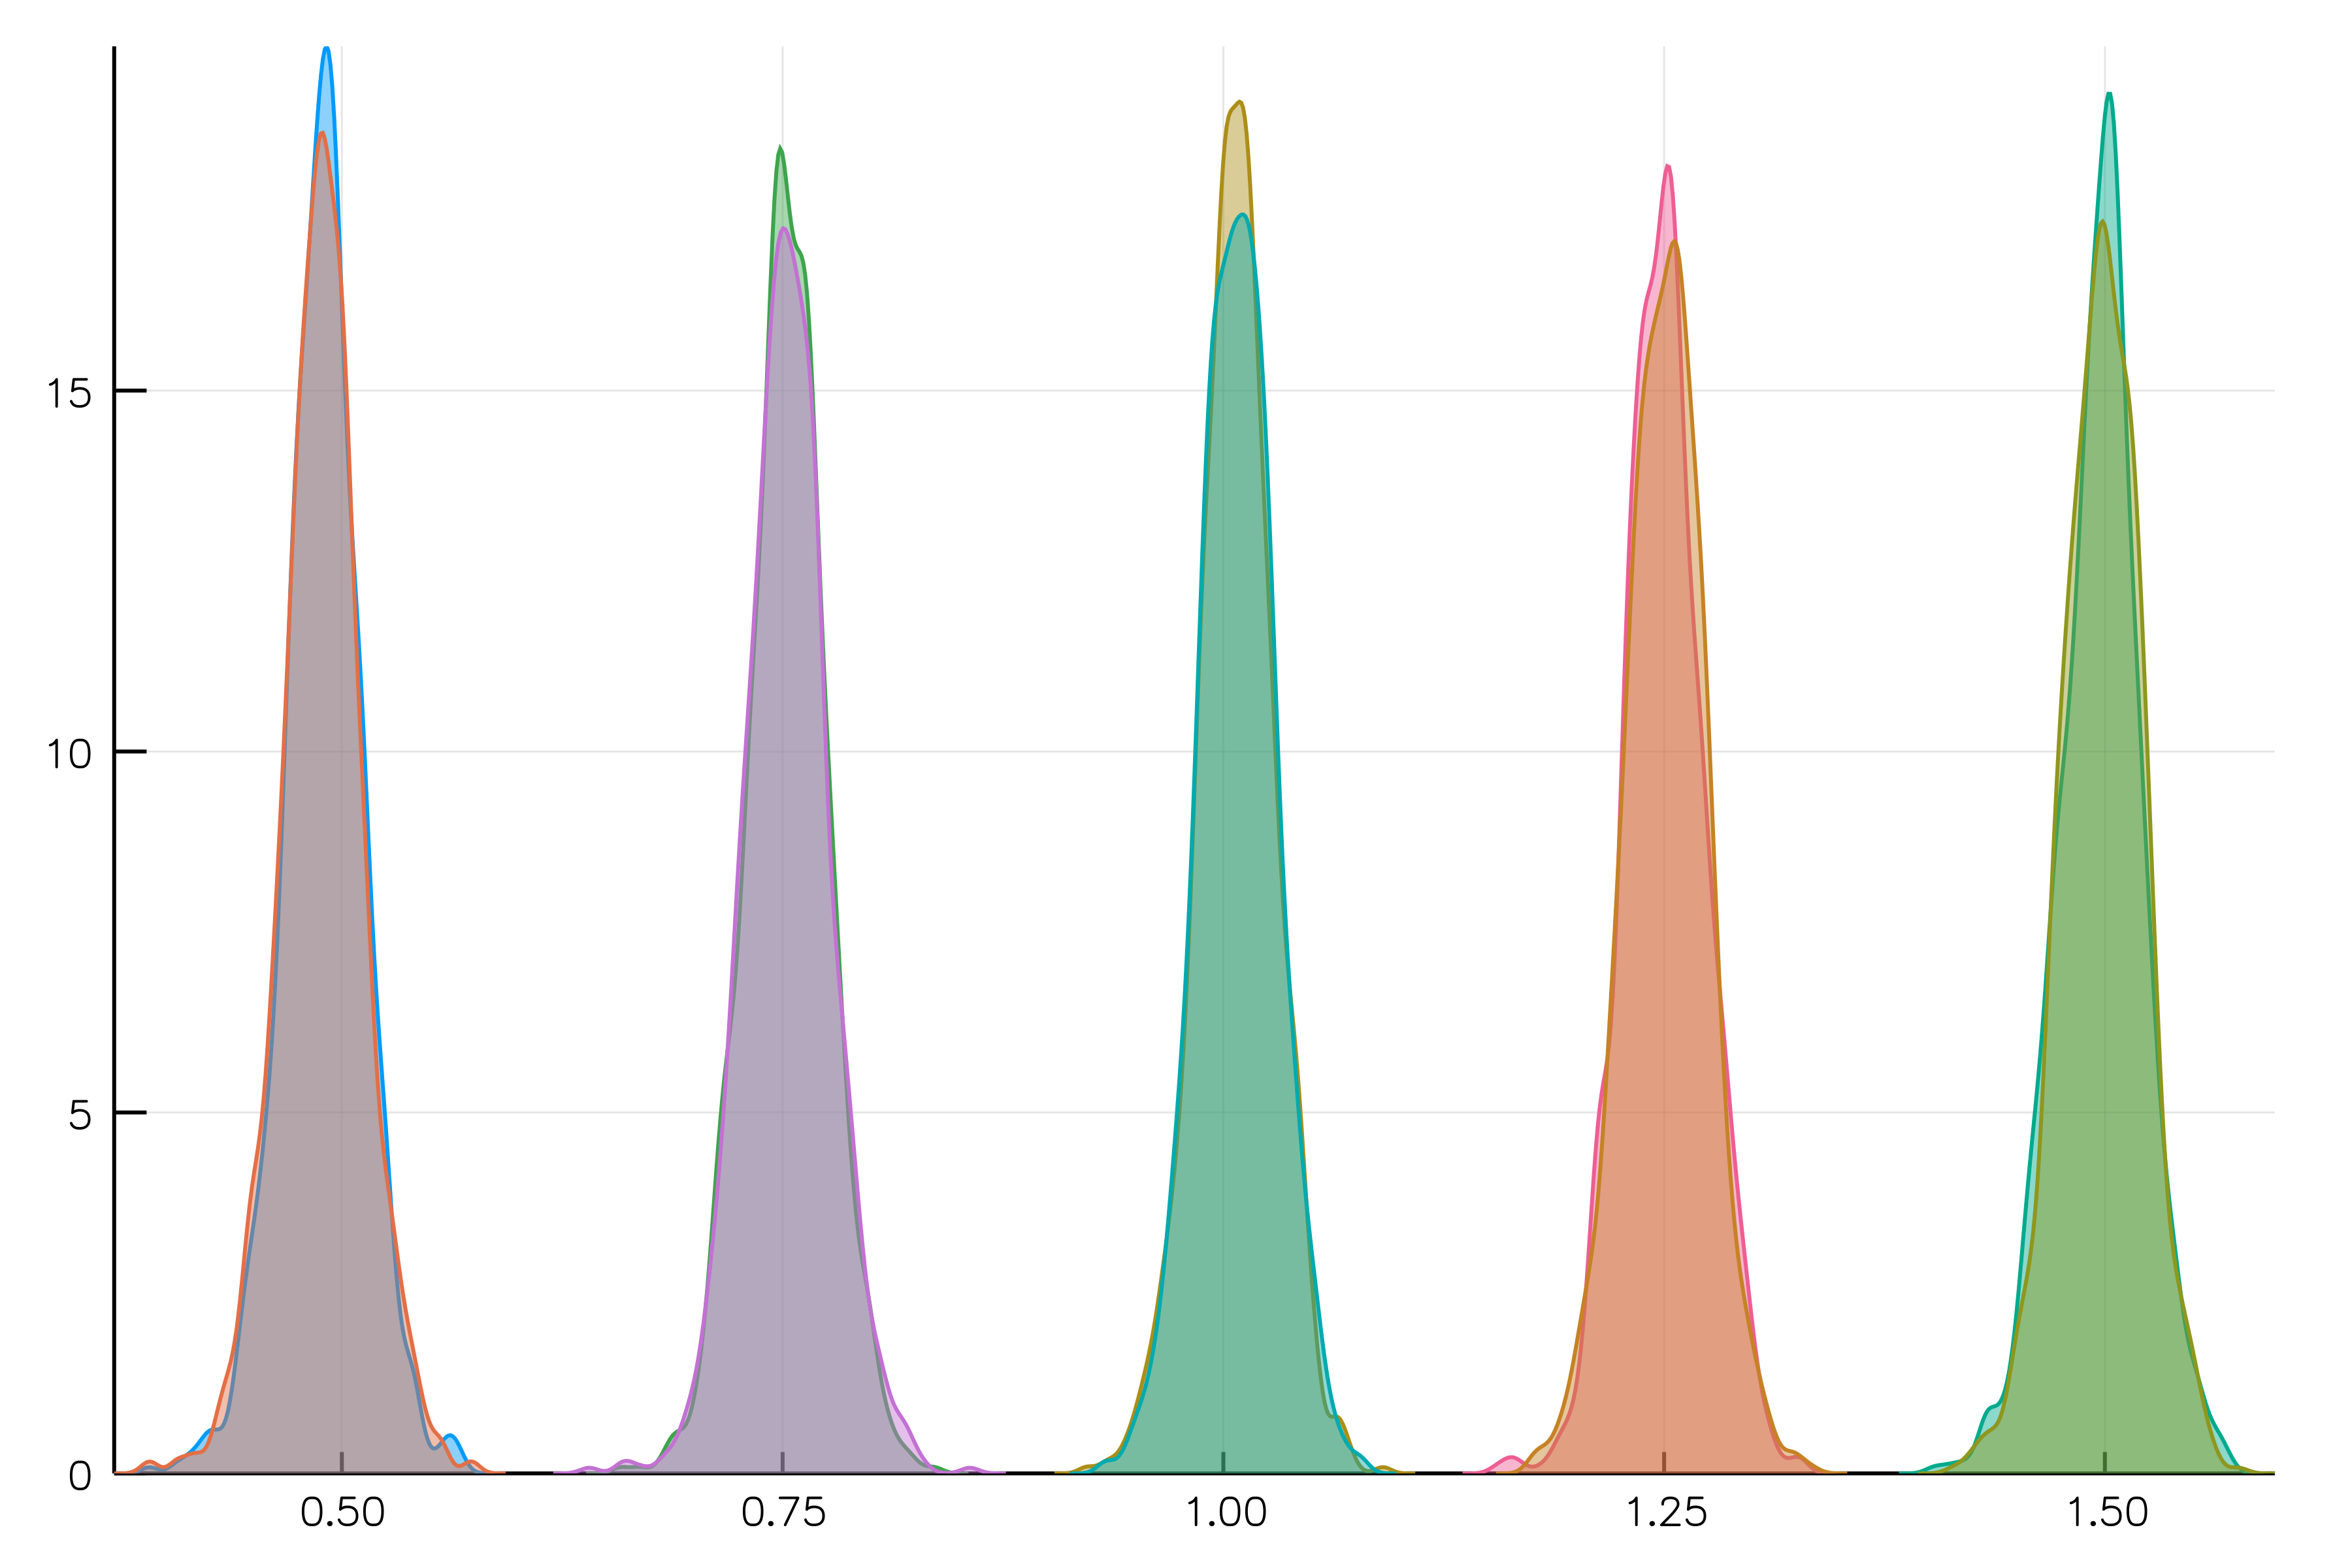
\includegraphics[width = 0.85\textwidth]{Levels}
	\caption{Distribution of Parameter Estimates (1,000 replications)}
	\label{LowLevel}
\end{figure}

Given a set of suitable conditions, it is possible to learn the true cluster structure from a proxy that has high purity, but at an incorrect level. The technique requires that each sub-cluster has enough power to provide consistent estimates (e.g., a pair of observations or household level might not provide enough observations). For example, observations that are located in a hierarchical setting such as county-state, could have a cluster structure at some unknown level. The county level presents a potential high-purity proxy, but would lead to a model with a great number of parameter estimates. In addition, it may be that the population distribution not accurately estimated at the county level. One potential way to construct a suitable proxy would be to estimate the model with the proxy at the county level and test whether the parameter estimates of certain heterogeneous parameters are the same (e.g., F-test). One can re-estimate the models until each heterogeneous in treatment parameter has been identified which leads to a parsimonious yet robust model.

In certain cases, a proxy may be given by more than one dimension. For example, an heterogeneous in treatment parameter may be a function of the state and the year. In this case, the high-purity proxy would be the combination of state and year; one could use the procedure described above to obtain a parsimonious and robust proxy in said case.

\FloatBarrier
\section{Analysis of Dimensional Accuracy Conditions}

A cluster robust model requires a suitable proxy for each heterogeneous in treatment parameter. A proxy can either be correct (robust and parsimonious), at the wrong level (robust), or impure (inconsistent). Given a representative sample and non-clustered sampling design, regardless of chosen proxy, an homogeneous in treatment parameter will be robust. Moreover, with sufficient power, one can identify the parameter as homogeneous since all estimates will have the same probability limit. In the case of heterogeneous in treatment parameters, one can apply a high-purity or an impure proxy.

Practitioners may face the problem where a potential heterogeneous in treatment parameter could have a cluster structure dependent on more than one possible dimension. For example, support for welfare programs could be heterogeneous in treatment by age, political ideology or some combination. The first step is to identify if the sampling cluster is clustered by any of the dimensions. If the sampling design is not clustered, a consistent estimator for the average partial effect in the population can be obtained if the samples are representative (both in cluster composition and cluster-specific distribution of attributes). In the case that the sampling design is clustered in a dimension that can pose an issue requiring a cluster robust model, the following guidelines can help. (1) If the dimension is unrelated to the cluster structure, the parameter estimates should converge to the same probability limit. (2) If the parameter estimates differ statistically, modify the cluster structure to a higher expected purity level for testing whether the cluster structure is at the wrong level.

\FloatBarrier

\section{Conclusion}

One contribution of this study is an alternative solution to cluster robust variance covariance estimators which relies on the assumptions used for such estimator about the data generation process and sampling design. In the case that one suspects or cares about heterogeneity in treatment effects in one dimension and has an available proxy for the subgroups, one could estimate a full interaction model between the variable and the subgroups which provide the better estimates for the parameters and information for Wald-test applications such as hypothesis testing.

Cluster robust models offer a way to consistently estimate average marginal effects for heterogeneous in treatment effects with clustered sampling design. These models rely on estimating cluster structures for the various parameters of the model that can be used to obtained consistent estimates of the heterogeneous in treatment effects. This study is the first to relax the unrealistic perfect information assumption and consider the various implications of having an imperfect cluster structure proxy. It shows that proxies can be understood within a framework of purity, level, and dimension. Purity relates to accurately each observation is correctly labeled, level considers if clusters should be aggregated, and the dimension offers tools to diagnose and improve proxies.

Obtaining a high purity proxy yields a consistent and possibly parsimonious solution. Defining the cluster structure at the wrong level yields consistent estimates, but overly-complicated model and requires more information about the population cluster structure than a parsimonious solution. Impure clusters provide inconsistent estimates for heterogeneous in treatment parameters. Under certain conditions, defining a theorized high-purity proxy can be used to identify impure proxies or prune clusters to obtain a more parsimonious, yet robust model.

\printbibliography

\appendix

\section{Code}

\end{document}